\documentclass[border=1pt]{standalone}
\usepackage{pgfplots}
\usepgfplotslibrary{groupplots,fillbetween}
\usepackage{animate}

\usepackage{pgf}
\usepackage{tikz}

\usetikzlibrary{fit}
\usetikzlibrary{positioning}
\usetikzlibrary{arrows}
\usetikzlibrary{automata}
\usetikzlibrary{backgrounds}
\usetikzlibrary{shapes.misc}

% https://tex.stackexchange.com/questions/118223/drawing-little-semicircle-to-show-that-two-intersecting-lines-are-not-connected
\usetikzlibrary{calc}

% \intersect{<p1>}{<p2>}{<q1>}{<q2>}
% draws the line p1--p2, showing a little semicircle
% where it intersects the line q1--q2.
\newcommand\intersect[4]{
  \draw let \p{c} = (intersection of #1--#2 and #3--#4) in
    (#1) -- ($(\p{c})!0.75mm!(#1)$) 
    to[bend right=90] ($(\p{c})!0.75mm!(#2)$) -- (#2)
}


\begin{document}    

 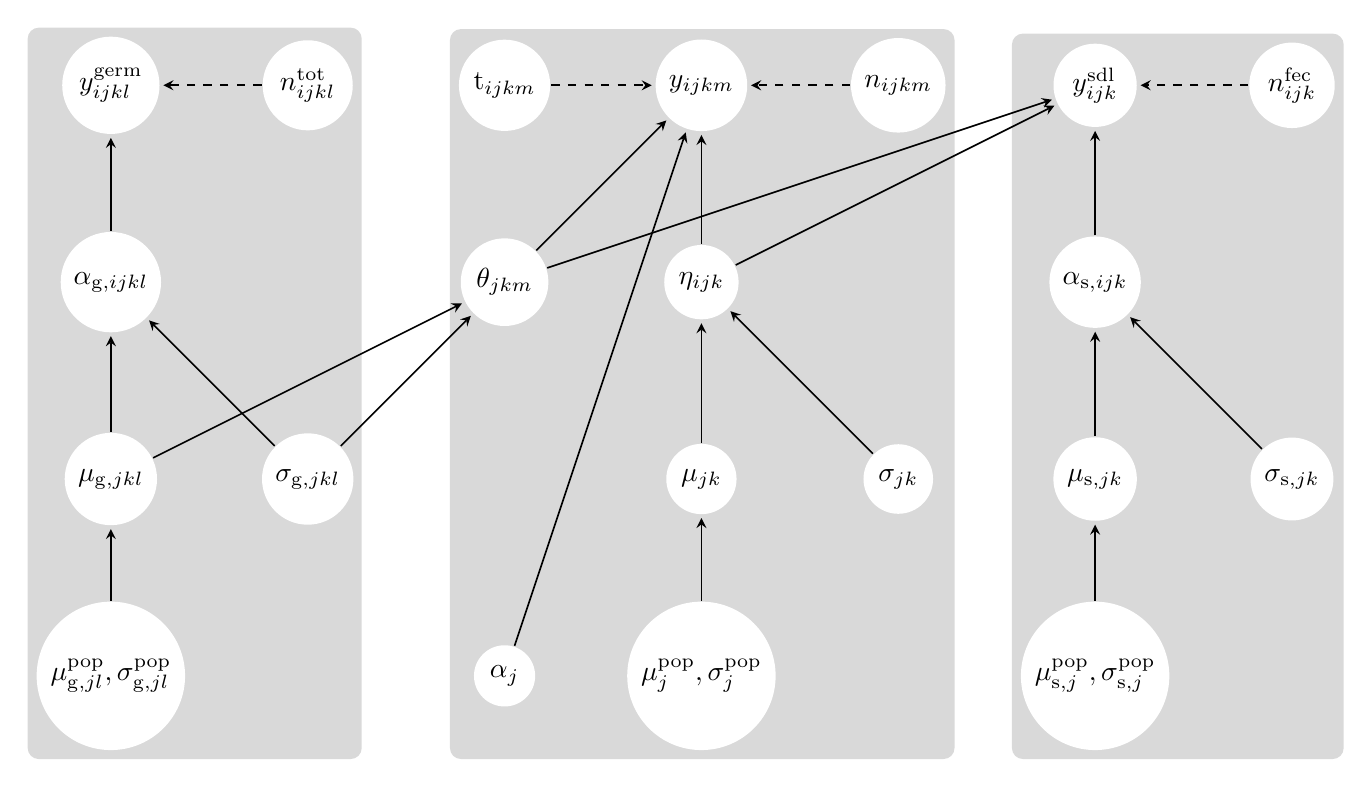
\begin{tikzpicture}[
            > = stealth, % arrow head style
            shorten > = 1pt, % don't touch arrow head to node
            auto,
            node distance = 2.5cm, % distance between nodes
            semithick, % line style
            scale=1
        ]

        \tikzstyle{every state}=[
            draw = none,
            thick,
            fill = white,
            minimum size = 4mm
        ]


	% data level
        \node[state] (Y) [] {$y^{\mathrm{germ}}_{ijkl}$};
        \node[state] (N) [right of=Y] {$n^{\mathrm{tot}}_{ijkl}$};
       
        \path[dashed,->] (N) edge node {} (Y);
                  
         % hyperparameters
         \node[state] (AB) [below of = Y] {$\alpha_{\mathrm{g},ijkl}$};
                
         \path[->] (AB) edge node {} (Y);
         
          % hyperparameters
        
         \node[state] (MS) [below of = AB] {$\mu_{\mathrm{g},jkl}$};
         \node[state] (A)[ right of = MS]  {$\sigma_{\mathrm{g},jkl}$};
         
         \path[->] (A) edge node {} (AB);       
         \path[->] (MS) edge node {} (AB);       
         
         \node[state] (H) [below of = MS] {$\mu^\mathrm{pop}_{\mathrm{g},jl},\sigma^\mathrm{pop}_{\mathrm{g},jl}$};
         \path[->] (H) edge node {} (MS);       
          
         %% SURVIVAL

	% data level
        \node[state] (T2) [right of = N] {$\mathrm{t}_{ijkm}$};
        \node[state] (Y2) [right of = T2] {$y_{ijkm}$};
        \node[state] (N2) [right of=Y2] {$n_{ijkm}$};

        \path[dashed,->] (N2) edge node {} (Y2);

        \path[dashed,->] (T2) edge node {} (Y2);

                  % hyperparameters
        \node[state] (AB2) [below of = Y2] {$\eta_{ijk}$};
       \node[state] (TH2) [left of = AB2] {$\theta_{jkm}$};
        
         \path[->] (AB2) edge node {} (Y2);
         \path[->] (TH2) edge node {} (Y2);
         \path[->] (MS) edge node {} (TH2);
          \path[->] (A) edge node {} (TH2);
                  
          % hyperparameters
        
         \node[state] (MS2) [below of = AB2] {$\mu_{jk}$};
         \node[state] (A2) [ right of = MS2]  {$\sigma_{jk}$};
         
         \path[->] (A2) edge node {} (AB2);       
         \path[->] (MS2) edge node {} (AB2);       
         
         \node[state] (H2) [below of = MS2] {$\mu^\mathrm{pop}_{j},\sigma^\mathrm{pop}_{j}$};
         \path[->] (H2) edge node {} (MS2);       
         
         \node[state] (ALPHA2) [left of = H2] {$\alpha_{j}$};
         \path[->] (ALPHA2) edge node {} (Y2);       

         % INITIAL SURVIVAL

	% data level
        \node[state] (Y3) [right of =N2] {$y^{\mathrm{sdl}}_{ijk}$};
        \node[state] (N3) [right of=Y3] {$n^{\mathrm{fec}}_{ijk}$};
       
        \path[dashed,->] (N3) edge node {} (Y3);
                   
        % hyperparameters
         \node[state] (AB3) [below of = Y3] {$\alpha_{\mathrm{s},ijk}$};
               
         \path[->] (AB3) edge node {} (Y3);
         \path[->] (AB2) edge node {} (Y3);
         \path[->] (TH2) edge node {} (Y3);
        
          % hyperparameters
        
         \node[state] (MS3) [below of = AB3] {$\mu_{\mathrm{s},jk}$};
         \node[state] (A3)[ right of = MS3]  {$\sigma_{\mathrm{s},jk}$};
         
         \path[->] (A3) edge node {} (AB3);       
         \path[->] (MS3) edge node {} (AB3);       
         
         \node[state] (H3) [below of = MS3] {$\mu^\mathrm{pop}_{\mathrm{s},j},\sigma^\mathrm{pop}_{\mathrm{s},j}$};
         \path[->] (H3) edge node {} (MS3);       
         
         
         % BACKGROUND

   \begin{scope}[on background layer]
   \node [fit=(T2) (N2) (H2), fill= gray!30, rounded corners, inner sep=.1cm] {};
   \node [fit=(Y) (N) (H), fill= gray!30, rounded corners, inner sep=.1cm] {};
   \node [fit=(Y3) (N3) (H3), fill= gray!30, rounded corners, inner sep=.1cm] {};
  \end{scope}
  
  \end{tikzpicture}

  
  \end{document}